\chapter{Implementation}

  In recent work He et al. \cite{DBLP:journals/corr/abs-2005-02131} proposed the first link stealing attacks on graph neural networks.
  They focused on stealing links of the graph, that was used for training the given target model.
  Like described in Section 3.3.1 this is an attack on transductive trained graph neural networks.
  In our work, we want to show, that it is possible for an adversary to steal links from any graphs, given black-box access to an inductive trained target graph neural network model.

  \textbf{Adversary's Goal}

  Let $f$ be the target graph neural network model and $G_{adv} = (V_{adv}, E_{adv})$ a graph with $|V_{adv}|$ nodes and $|E_{adv}|$ edges. 
  We assume, that some of $G_{adv}$'s links/edges are missing.
  The goal of an adversary is, to infer whether two nodes $i$ and $j$ are connected to each other or not.
  More precisely, whether the link $(i,j)$ between node $i$ and node $j$ is missing or does not exist.
  

  \section{Attack 1}

    In this section, we propose our first attack. 
    Given a target graph neural network model $f$ and a graph $G_{adv}$ of the same dataset distribution as $f$'s training graph, an adversary $a$ aims to steal missing edges of $G_{adv}$.
    Therefor it uses the posterior output $f(i)$ and $f(j)$ of two nodes $i$ and $j$ and concatenates them to get the input feature $post_{ij} = concat(f(i),f(j))$. The adversary $a$ is then trained on $post_{ij}$.

    \subsection{Thread Model}

      In this attack the adversary $a$ has \emph{Black-Box Access} (Query-Access) to the target model $f$. 
      The graph $G_{adv}$ is from the same dataset distribution. 
      However, $f$ wasn't trained on $G_{adv}$.

    \subsection{Attack Methodology}

      % DATASET PreProcessing:
      To perform this attack, we split a given dataset $G = (V, E)$, into one traingraph $G_{train} = (V_{train}, E_{train})$ and one testgraph $G_{test} = (V_{test}, E_{test})$.  
      We sample the traingraph as $V_{train} = \{i | \forall i \in V: random(0, 1) == 1\}$, where $random(0, 1)$ returns the values $0$ or $1$ at random, leading to a random split of the nodes.
      $E_{train} = \{(i, j) | \forall (i,j) \in E: i, j \in V_{train}\}$ now contains the edge $(i,j)$ if both nodes $i$ and $j$ are in $V_{train}$.
      The testgraph is now sampled similary.
      $V_{test} = \{j | \forall j \in V: j \not\in V_{train}\}$ and $E_{test} = \{(i, j) | \forall (i,j) \in E: i, j \in V_{test}\}$

      \subsubsection{Target Model}

        The target model $f$ is now trained on $G_{train}$ to perform a node classification task.
        Especially, given a node's features, its neighbors' and the edges between them, $f$ outputs a prediction posterior of the class.

      \subsubsection{Attacker Model}

        We first create a raw dataset $d_{raw}$ based on $G_{test}$.
        To do so, we create a clone of the testgraph $G_{adv} = G_{test}$, which will represent the adversary's graph.
        We now collect a set of positive samples $pos = \{(i,j, 1) | \forall i,j \in V_{test}: (i,j) \in E_{test} \wedge |pos| < ((1 - \alpha) * |E_{test}|))\}$, containing pairs of nodes, that are connected in the testgraph, where $\alpha$ denotes the percentage of known edges.
        We then delete all edges we sampled, in our graph clone $E_{adv} = \{(i,j) | \forall (i,j) \in E_{adv}: (i,j) \not\in pos\}$, to represent the missing edges, we want to steal.
        Now, we collect a set of negative samples $neg = \{(i,j, 0) | \forall i,j \in V_{test}: (i,j) \not\in E_{test} \wedge |neg| < ((1 - \alpha) * |E_{test}|))\}$, containing pairs of nodes, that are not connected in $G_{test}$.
        Our raw dataset \emph{da-raw} = $pos \cup neg$, now contains positive and negative samples obtained from $G_{test}$.
        As the next step, we create the adversary's dataset $da = \{(post_{ij}, l) | \forall (i,j,l)\in\emph{da-raw}: post_{ij} = concat(target(G_{adv}, i), target(G_{adv}, j))\}$.
        $target(G_adv, i)$ returns the node classification output posterior of the target model, when it is queried on $i$ given the adversary's graph $G_{adv}$.
        $concat(a, b)$ concatenates the output posteriors $a$ and $b$ with each other returning the feature we will train the attacker model on.
        $l$ denotes the label either being 1 (positive sample) or 0 (negative sample).
        With our adversary's dataset $da$ we can now continue training our attacker model using $post_{ij}$ as input features and $l$ as class.

  \section{Attack 2}

    In this section, we propose our second attack. Given a target graph neural network and a graph of the same dataset, that wasn't used for training the target model, an adversary aims to steal missing edges of its graph.
    Therefor it uses the posterior output of the two nodes, it queries the network on and calculates the distance between these two vectors in eight different ways and uses these values as input features for training the attacker model.

    % \begin{figure}[h!]
    % \begin{center}
    %   \subfloat{
    %     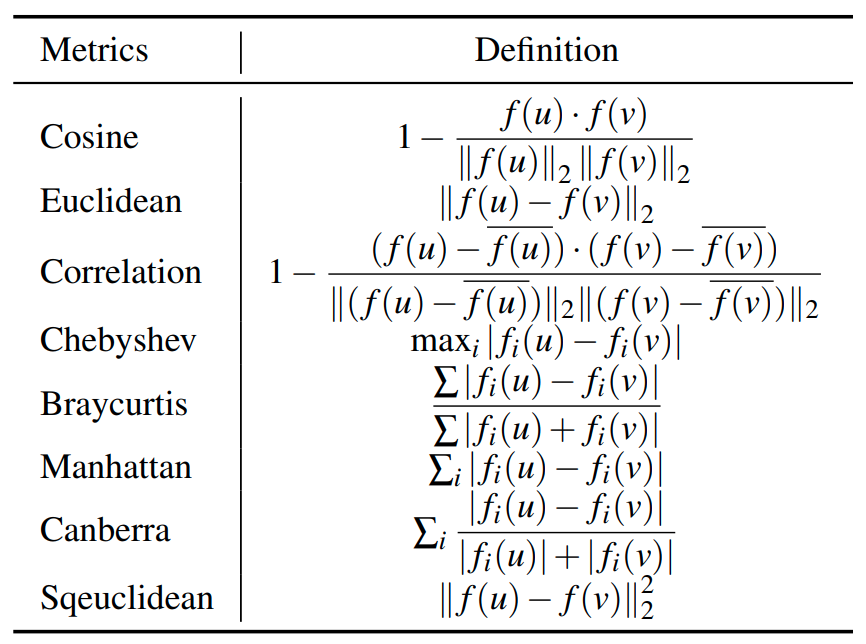
\includegraphics[scale=0.3]{res/Figures/distance-metrics}}
    %     \caption{This is an attacker}
    %     \end{center}
    % \end{figure}

    % \begin{center}
    %   \begin{table}[h!]
    %     \begin{tabular}{ll}
    %       Metrics     & Formal Definition \\
    %       Cosine      & $1 -\dfrac{\TargetModel(u)\cdot\TargetModel(v)}{\left|\TargetModel(u)\right|2\left|\TargetModel(v)\right|_2}$ \\
    %       Euclidean   & $\left|\TargetModel(u) - \TargetModel(v)\right|_2$ \\
    %       Correlation & $1-\dfrac{(\TargetModel(u)-\overline{\TargetModel(u)}) \cdot(\TargetModel(v)-\overline{\TargetModel(v)})}{|(\TargetModel(u)-\overline{\TargetModel(u)})|{2}|(\TargetModel(v)-\overline{\TargetModel(v)})|{2}}$ \\
    %       Chebyshev   & $\max _{i}\left|\TargetModel_i(u)-\TargetModel_i(v)\right|$ \\
    %       Braycurtis  & $\dfrac{\sum\left|\TargetModel_i(u)-\TargetModel_i(v)\right|} {\sum\left|\TargetModel_i(u)+\TargetModel_i(v)\right|}$ \\
    %       Manhattan   & $\sum{i}\left|\TargetModel_i(u)-\TargetModel_i(v)\right|$ \\
    %       Canberra    & $\sum_{i} \dfrac{\left|\TargetModel_i(u)-\TargetModel_i(v)\right|}{\left|\TargetModel_i(u)\right|+\left|\TargetModel_i(v)\right|}$ \\
    %       Sqeuclidean & $\left|\TargetModel(u) - \TargetModel(v)\right|_2^2$
    %     \end{tabular}
    %   \end{table}
    % \end{center}


    \subsection{Thread Model}

      The Thread Model for this attack is the same one described in Section 4.1.1.

    \subsection{Attack Methodology}

      Most of the Attack Methodology is the same as the one described in Section 4.1.2.
      There is one difference however.
      Instead of using the concatenation of the two output posteriors, we now use them as vectors, to calculate their distances in eight different ways.
      We have in total experimented with 8 common distance metrics: Cosine distance, Euclidean distance, Correlation distance, Chebyshev distance, Braycurtis distance, Canberra distance, Manhattan distance, and Square-euclidean distance.

      \subsubsection{Attacker}

        We first create \emph{da-raw} like described in Section 4.1.2.2.
        Our adversary's dataset can now be desribed as the following.
        $da = \{(dist_{ij}, l) | \forall (i,j,l)\in\emph{da-raw}: dist_{ij} = d(target(G_{adv}, i), target(G_{adv}, j))\}$, where $d(a,b) = concat(dist_1(a,b), ..., dist_8(a,b))$ and $l$ again denotes the label.
        With our adversary's dataset $da$ we can now continue training our attacker model using $dist_{ij}$ as input features and $l$ as class.

  \section{Attack 3}

    In this section, we propose our last attack. Given a target graph neural network and a graph of a different dataset, that wasn't used for training the target model, an adversary aims to steal missing edges of its graph.
    Therefor it uses the posterior output of the two nodes, it queries the network on and calculates the distance between these two vectors in eight different ways and uses these values as input features for training the attacker model.

    \subsection{Thread Model}

      In this attack the adversary has \emph{Black-Box Access} (Query-Access) to the target model and uses a different source dataset than the target.

    \subsection{Attack Methodology}

      As mentioned before, we now have two different datasets $G_{target} = (V_{target}, E_{target})$ and $G_{attacker\_model} = (V_{attacker\_model}, E_{attacker\_model})$.

      \subsubsection{Target}

        The target model is now trained on $G_{target}$ to perform node classification.
        Especially,given a node’s features, its neighbors’ and the edges between them, the model outputs aprediction posterior of the class.

      \subsubsection{Attacker Model}

        We first create the raw dataset \emph{da-raw} the same way, we did before but this time with $G_{attacker\_model}$.
        To do so, we again create a clone $G_{adv} = G_{attacker\_model}$.
        We now collect a set of positive samples $pos = \{(i,j, 1) | \forall i,j \in V_{attacker\_model}: (i,j) \in E_{attacker\_model} \wedge |pos| < ((1 - \alpha) * |E_{attacker\_model}|))\}$.
        We then delete all edges we sampled, in our graph clone $E_{attacker\_model} = \{(i,j) | \forall (i,j) \in E_{adv}: (i,j) \not\in pos\}$, to represent the missing edges, we want to steal.
        Now, we collect a set of negative samples $neg = \{(i,j, 0) | \forall i,j \in V_{attacker\_model}: (i,j) \not\in E_{test} \wedge |neg| < ((1 - \alpha) * |E_{attacker\_model}|))\}$, containing pairs of nodes, that are not connected in $G_{attacker\_model}$.
        Our raw dataset \emph{da-raw} = $pos \cup neg$, now contains positive and negative samples obtained from $G_{attacker\_model}$.
        As the next step, we create the adversary's dataset $da = \{(dist_{ij}, l) | \forall (i,j,l)\in\emph{da-raw}: dist_{ij} = d(target(G_{adv}, i), target(G_{adv}, j))\}$, where $d(a,b) = concat(dist_1(a,b), ..., dist_8(a,b))$ and $l$ again denotes the label.
        With our adversary's dataset $da$ we can now continue training our attacker model using $dist_{ij}$ as input features and $l$ as class.



  \section{Datasets}

  \section{Target Models}

    \subsection{GraphSAGE}

    \subsection{Graph Attention Networks}

    \subsection{Graph Convolutional Networks}

  \section{Attacker Model}
